\documentclass{beamer}
%
% Choose how your presentation looks.
%
% For more themes, color themes and font themes, see:
% http://deic.uab.es/~iblanes/beamer_gallery/index_by_theme.html
%
\mode<presentation>
{
  \usetheme{Madrid}      % or try Darmstadt, Madrid, Warsaw, ...
  \usecolortheme{wolverine} % or try albatross, beaver, crane, ...
  \usefonttheme{default}  % or try serif, structurebold, ...
  \setbeamertemplate{navigation symbols}{}
  \setbeamertemplate{caption}[numbered]
} 

\usepackage[english]{babel}
\usepackage[utf8x]{inputenc}
\usepackage{graphicx}
\title[Un webservice pour BiBler]{Présentation de projet - IFT3150}
\author{Félix Bélanger-Robillard}
\institute{DIRO}
\date{2017-04-26}

\begin{document}

\begin{frame}
  \titlepage
\end{frame}

% Uncomment these lines for an automatically generated outline.
%\begin{frame}{Outline}
%  \tableofcontents
%\end{frame}

\section{Introduction}

\begin{frame}{Introduction}

\begin{itemize}
  \item But du projet: mettre BiBler en webservice
  \item Intégration avec ReLis
\end{itemize}


\end{frame}

\begin{frame}{Plan de la Présentation}

\begin{enumerate}
  \item Introduction
  \item Terminologie
  \item Analyse des besoins
  \item Conception
  \item Design
  \item Implémentation
  \item Tests et documentation
  \item Intégration et déploiement
  \item Maintenance
  \item Conclusion
  \item Questions
\end{enumerate}

\end{frame}

\begin{frame}{Terminologie}

\begin{block}{BiBler}
Logiciel de gestion de références
\end{block}

\begin{block}{ReLiS}
Système de Revue Littéraire Systématique. Logiciel web utilisant le framework CodeIgniter.
\end{block}

\end{frame}

\begin{frame}{Analyse des besoins}

\begin{block}{BiBler} 
\begin{itemize}
  \item Conserver au minimum les dépendances technologiques
  \item Déploiement possible sur Apache
\end{itemize}
\end{block}

\begin{block}{ReLiS} 
\begin{itemize}
  \item Ajouter Abstract au BiBtex
  \item Générer les clés
  \item Formatter les BibTeX
\end{itemize}
\end{block}


\end{frame}


\begin{frame}{Conception}

\begin{itemize}
  \item Instances localisées de BibLerApp
  \item Handler pour les requêtes client, Wrapper pour accéder à l'API
  \item Proxy pour accéder à partir de PHP
  \item Utilisation de web.py
\end{itemize}


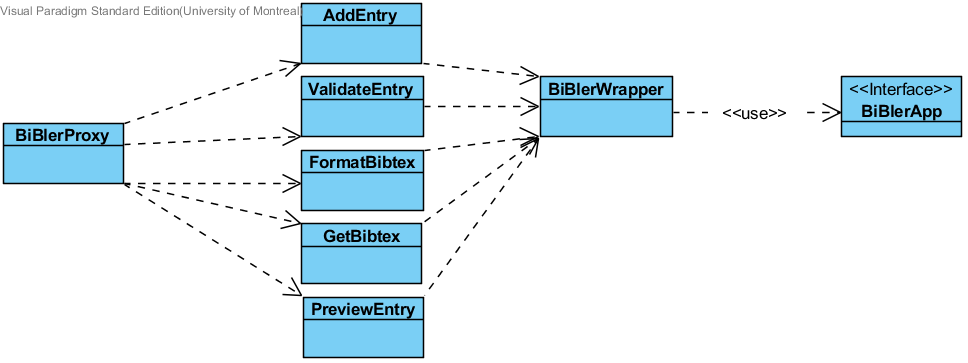
\includegraphics[width=\linewidth,height=\textheight,keepaspectratio]{DomainClassDiagram.png}


\end{frame}
\begin{frame}{Design}

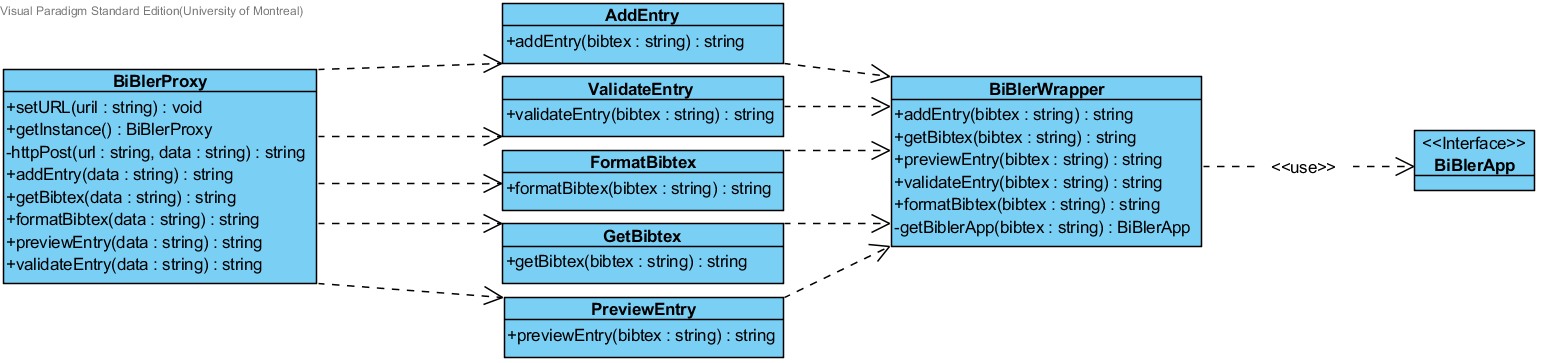
\includegraphics[width=\linewidth,height=\textheight,keepaspectratio]{ClassDiagram.png}
\end{frame}

\begin{frame}{Design}
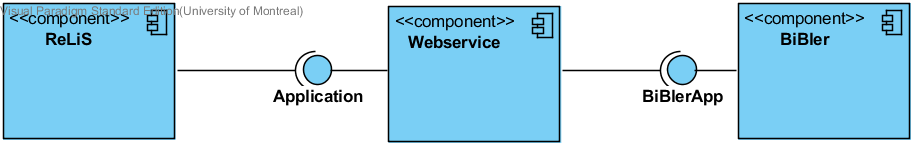
\includegraphics[width=\linewidth,height=\textheight,keepaspectratio]{ComponentDiagram.png}
\end{frame}
\begin{frame}{Implémentation}

\begin{itemize}
  \item Regard sur l'application Python
  \item Regard sur PHP
  \item Regard sur ReLiS
\end{itemize}
\end{frame}
\begin{frame}{Tests et documentation}

\begin{itemize}
  \item Regard sur les test unitaires
  \item Performance
  \item Documentation Sphinx
\end{itemize}

\end{frame}
\begin{frame}{Performance}
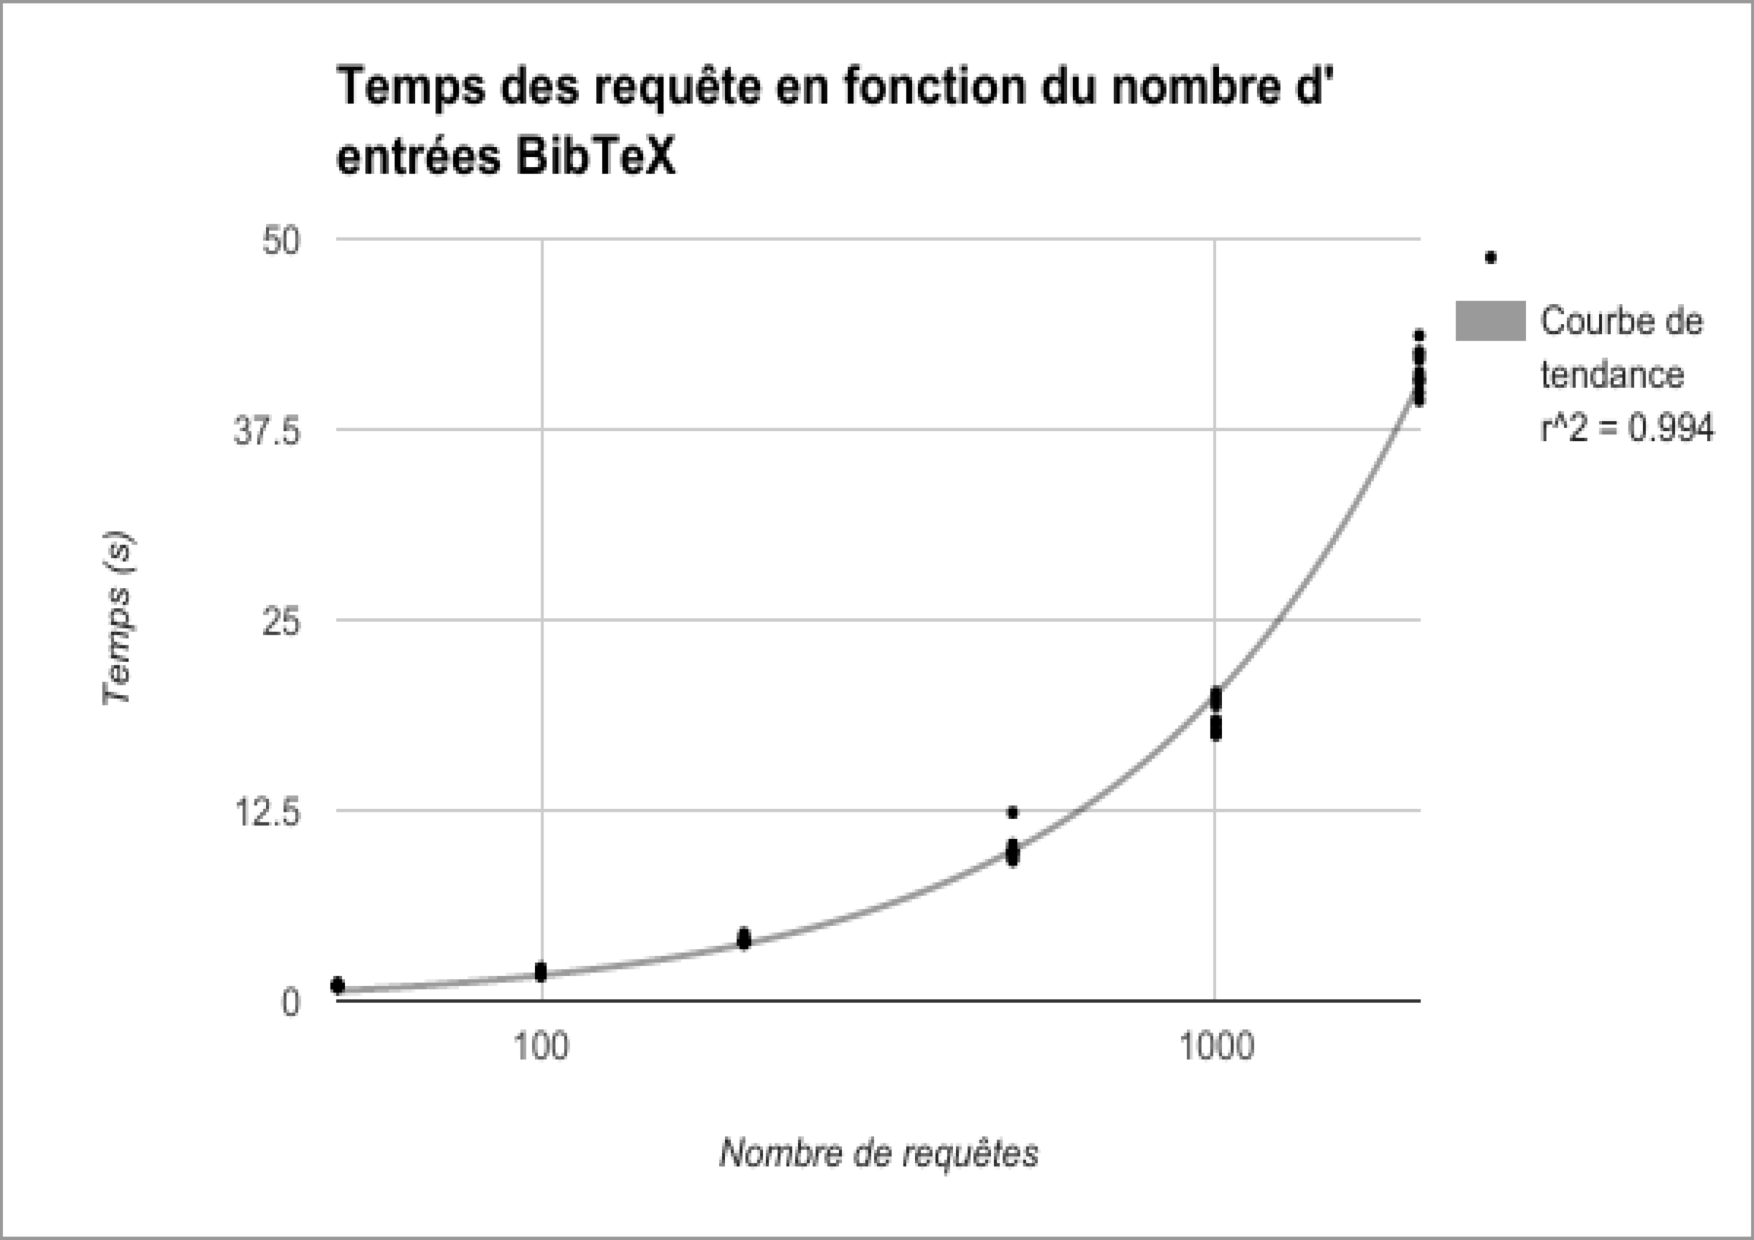
\includegraphics[width=\linewidth,height=\textheight,keepaspectratio]{tempsparrequete.pdf}
\end{frame}

\begin{frame}{Performance}
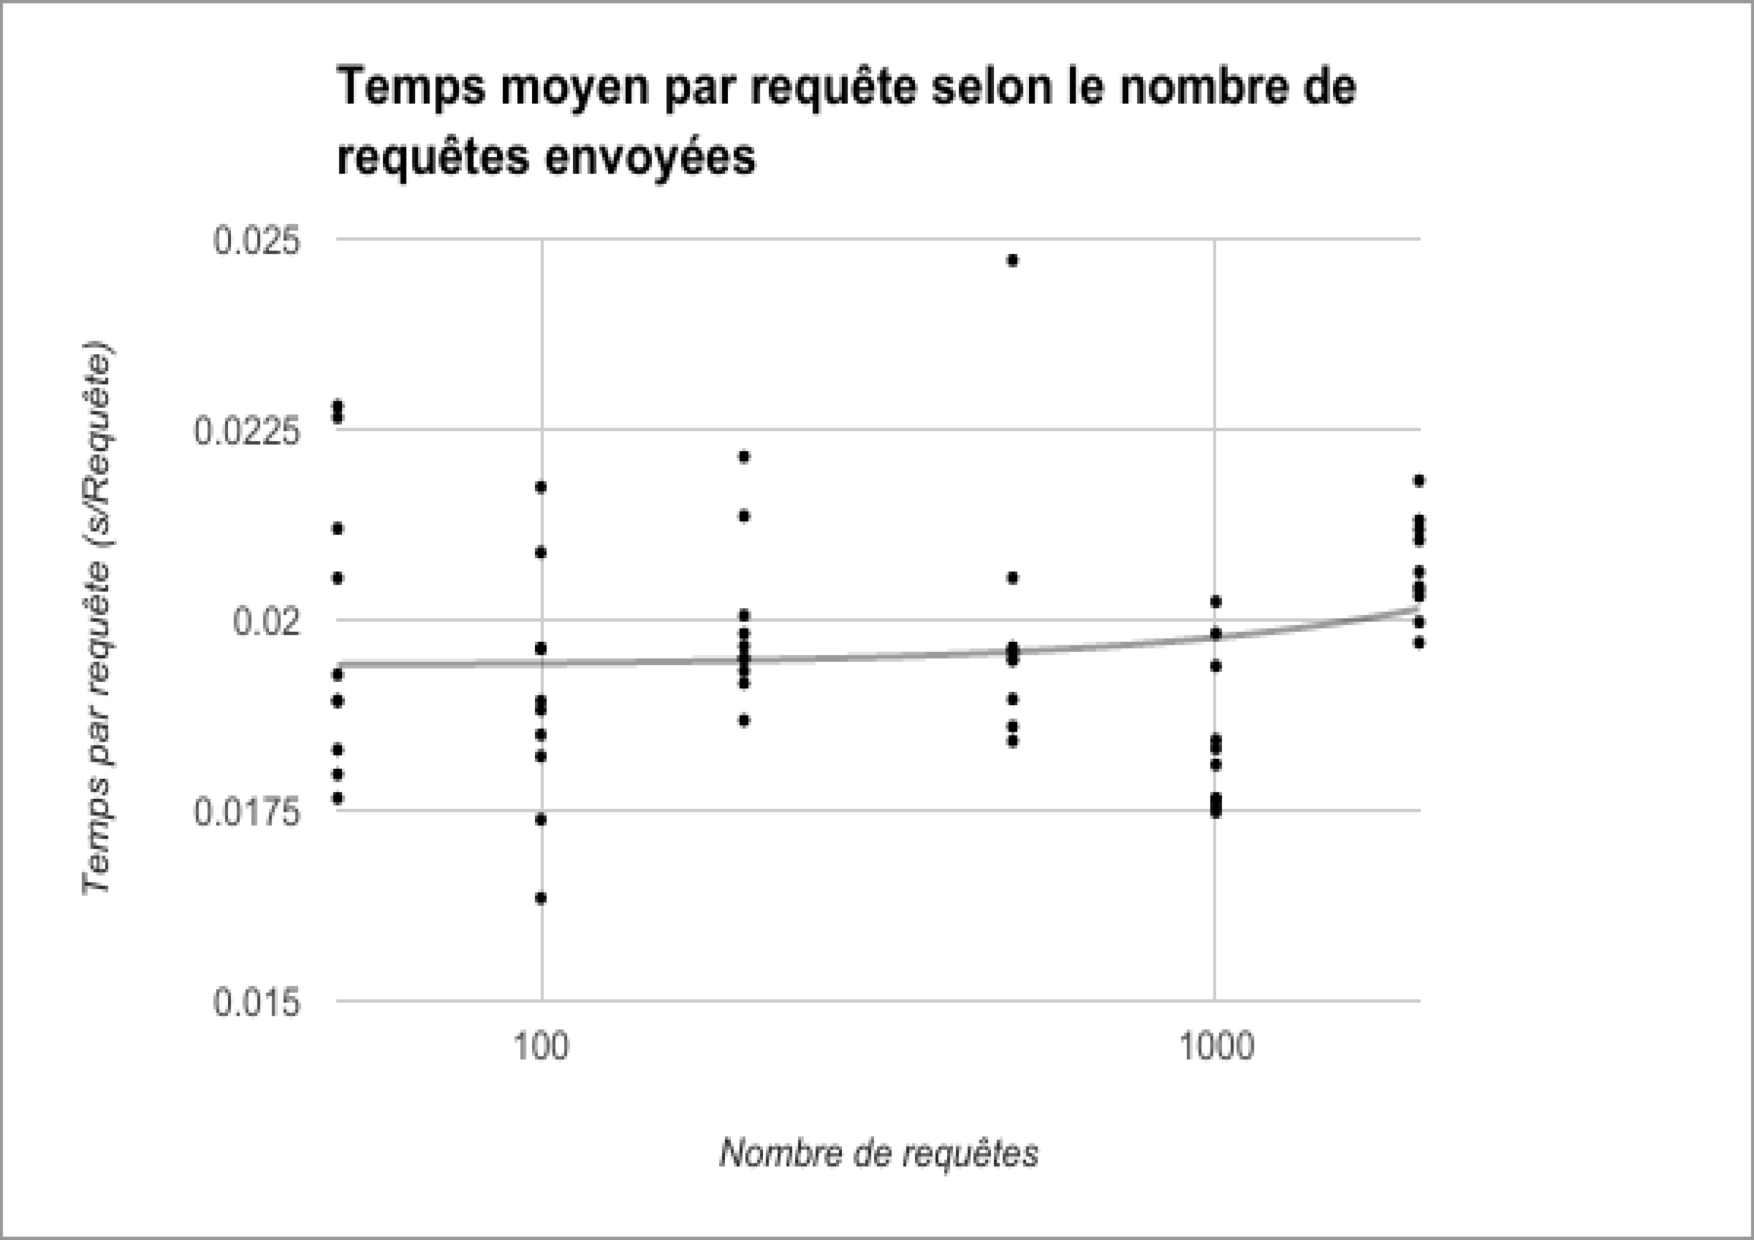
\includegraphics[width=\linewidth,height=\textheight,keepaspectratio]{tempsparequeteparrequete.pdf}
\end{frame}

\begin{frame}{Intégration et déploiement}

\begin{block}{Configuration du webservice} 
\begin{itemize}
  \item Apache 2.4
  \item mod\_wsgi pour Apache
  \item PHP 5.5
  \item En attente de la disponibilité du serveur
\end{itemize}
\end{block}

\end{frame}

\begin{frame}{Maintenance}
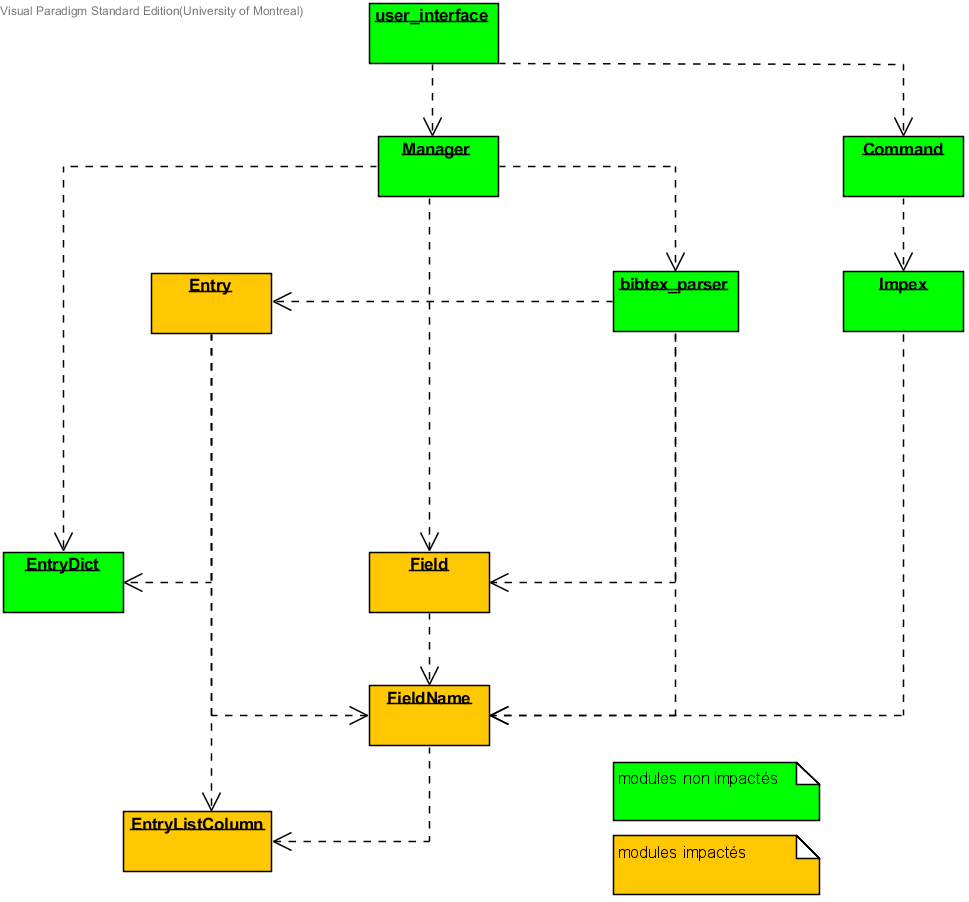
\includegraphics[width=\linewidth,height=0.8\textheight,keepaspectratio]{impact.png} 
\end{frame}

\begin{frame}{Maintenance}
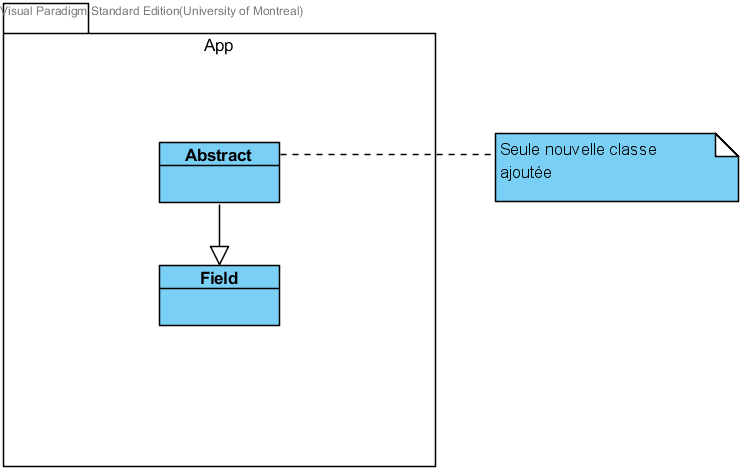
\includegraphics[width=\linewidth,height=\textheight,keepaspectratio]{maintenance.png}
\end{frame}


\begin{frame}{Conclusion}
\begin{itemize}
  \item Webservice complété
  \item Intégration incomplète, mais Proxy disponible
  \item Performances stables
\end{itemize}

\end{frame}


\begin{frame}{Période de questions}

\end{frame}

\section{Some \LaTeX{} Examples}

\subsection{Tables and Figures}

\begin{frame}{Tables and Figures}

\begin{itemize}
\item Use \texttt{tabular} for basic tables --- see Table~\ref{tab:widgets}, for example.
\item You can upload a figure (JPEG, PNG or PDF) using the files menu. 
\item To include it in your document, use the \texttt{includegraphics} command (see the comment below in the source code).
\end{itemize}

% Commands to include a figure:
%\begin{figure}
%\includegraphics[width=\textwidth]{your-figure's-file-name}
%\caption{\label{fig:your-figure}Caption goes here.}
%\end{figure}

\begin{table}
\centering
\begin{tabular}{l|r}
Item & Quantity \\\hline
Widgets & 42 \\
Gadgets & 13
\end{tabular}
\caption{\label{tab:widgets}An example table.}
\end{table}

\end{frame}

\subsection{Mathematics}

\begin{frame}{Readable Mathematics}

Let $X_1, X_2, \ldots, X_n$ be a sequence of independent and identically distributed random variables with $\text{E}[X_i] = \mu$ and $\text{Var}[X_i] = \sigma^2 < \infty$, and let
$$S_n = \frac{X_1 + X_2 + \cdots + X_n}{n}
      = \frac{1}{n}\sum_{i}^{n} X_i$$
denote their mean. Then as $n$ approaches infinity, the random variables $\sqrt{n}(S_n - \mu)$ converge in distribution to a normal $\mathcal{N}(0, \sigma^2)$.

\end{frame}

\end{document}
